\documentclass[11pt,a4paper]{report}
\usepackage[utf8x]{inputenc}
\usepackage{ucs}
\usepackage[english]{babel}
\usepackage{amsmath}
\usepackage{amsfonts}
\usepackage{amssymb}
\usepackage{makeidx}
\usepackage{graphicx}
\usepackage{lmodern}
\usepackage[left=2cm,right=2cm,top=2cm,bottom=2cm]{geometry}
\author{Floor Broekgaarden}
\title{Master Project progress}

\begin{document}
\maketitle





\chapter{General adaptive importance sampling method }





The errors are given by 

Monte Carlo: 

\begin{equation}
	\sigma = std{\phi(x)}
	\label{eq:MC-error}
\end{equation}
%
\begin{equation}
	\sigma = std{\phi(x) \frac{p(x)}{g(x)}}
	\label{eq:AIS-error}
\end{equation}
%



\begin{figure}
	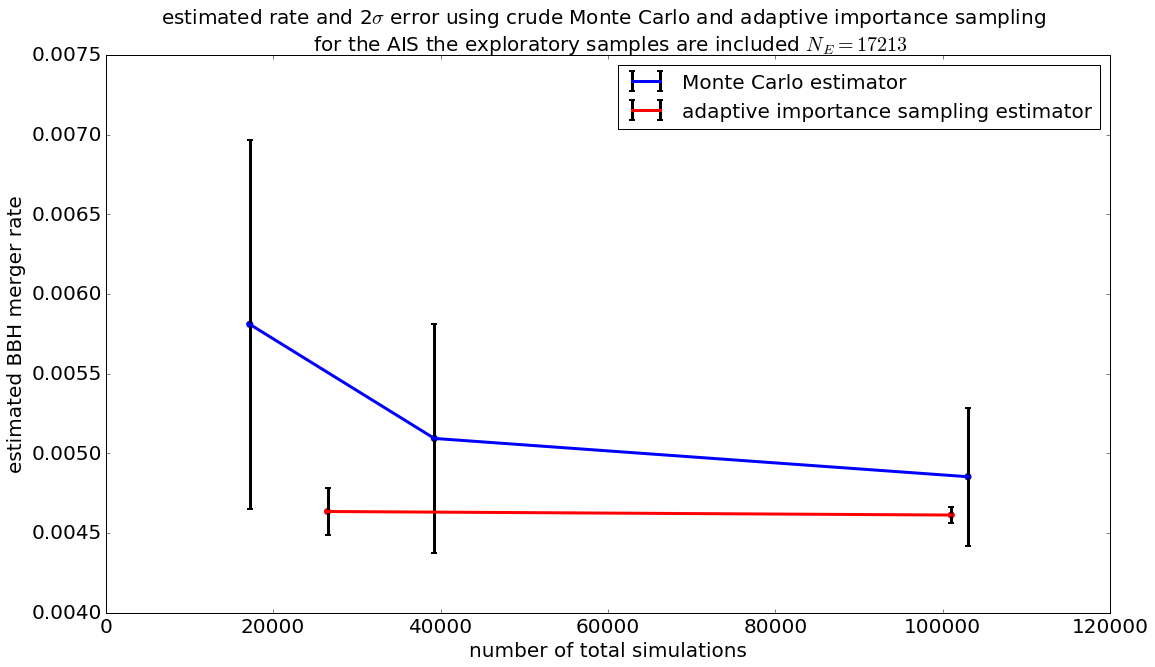
\includegraphics[width=\columnwidth]{bbhrate_error_evolution.png}
    \caption{First idea of what a plot could look like that shows the convergence of the Adaptive importance sampling method vs the Monte Carlo method. Shown here are the BBH merger rate estimated using (blue) crude Monte Carlo sampled simulation and (red) using adaptive importance sampling sampled simulation. The x-axes shows the total number of simulations that is used for the estimation and the y-axes shows the estimated rate. Plotted in black are the estimated errors for the simulations.}
    \label{fig:aIS_scheme}
\end{figure}
%



\chapter{Variations on adaptive importance sampling}

\chapter{Astrophysical details}

\chapter{Mathematical details}


\chapter{Planning and To do:}



\end{document}